\documentclass[twoside]{book}

% Packages required by doxygen
\usepackage{fixltx2e}
\usepackage{calc}
\usepackage{doxygen}
\usepackage[export]{adjustbox} % also loads graphicx
\usepackage{graphicx}
\usepackage[utf8]{inputenc}
\usepackage{makeidx}
\usepackage{multicol}
\usepackage{multirow}
\PassOptionsToPackage{warn}{textcomp}
\usepackage{textcomp}
\usepackage[nointegrals]{wasysym}
\usepackage[table]{xcolor}

% Font selection
\usepackage[T1]{fontenc}
\usepackage[scaled=.90]{helvet}
\usepackage{courier}
\usepackage{amssymb}
\usepackage{sectsty}
\renewcommand{\familydefault}{\sfdefault}
\allsectionsfont{%
  \fontseries{bc}\selectfont%
  \color{darkgray}%
}
\renewcommand{\DoxyLabelFont}{%
  \fontseries{bc}\selectfont%
  \color{darkgray}%
}
\newcommand{\+}{\discretionary{\mbox{\scriptsize$\hookleftarrow$}}{}{}}

% Page & text layout
\usepackage{geometry}
\geometry{%
  a4paper,%
  top=2.5cm,%
  bottom=2.5cm,%
  left=2.5cm,%
  right=2.5cm%
}
\tolerance=750
\hfuzz=15pt
\hbadness=750
\setlength{\emergencystretch}{15pt}
\setlength{\parindent}{0cm}
\setlength{\parskip}{3ex plus 2ex minus 2ex}
\makeatletter
\renewcommand{\paragraph}{%
  \@startsection{paragraph}{4}{0ex}{-1.0ex}{1.0ex}{%
    \normalfont\normalsize\bfseries\SS@parafont%
  }%
}
\renewcommand{\subparagraph}{%
  \@startsection{subparagraph}{5}{0ex}{-1.0ex}{1.0ex}{%
    \normalfont\normalsize\bfseries\SS@subparafont%
  }%
}
\makeatother

% Headers & footers
\usepackage{fancyhdr}
\pagestyle{fancyplain}
\fancyhead[LE]{\fancyplain{}{\bfseries\thepage}}
\fancyhead[CE]{\fancyplain{}{}}
\fancyhead[RE]{\fancyplain{}{\bfseries\leftmark}}
\fancyhead[LO]{\fancyplain{}{\bfseries\rightmark}}
\fancyhead[CO]{\fancyplain{}{}}
\fancyhead[RO]{\fancyplain{}{\bfseries\thepage}}
\fancyfoot[LE]{\fancyplain{}{}}
\fancyfoot[CE]{\fancyplain{}{}}
\fancyfoot[RE]{\fancyplain{}{\bfseries\scriptsize Generated by Doxygen }}
\fancyfoot[LO]{\fancyplain{}{\bfseries\scriptsize Generated by Doxygen }}
\fancyfoot[CO]{\fancyplain{}{}}
\fancyfoot[RO]{\fancyplain{}{}}
\renewcommand{\footrulewidth}{0.4pt}
\renewcommand{\chaptermark}[1]{%
  \markboth{#1}{}%
}
\renewcommand{\sectionmark}[1]{%
  \markright{\thesection\ #1}%
}

% Indices & bibliography
\usepackage{natbib}
\usepackage[titles]{tocloft}
\setcounter{tocdepth}{3}
\setcounter{secnumdepth}{5}
\makeindex

% Hyperlinks (required, but should be loaded last)
\usepackage{ifpdf}
\ifpdf
  \usepackage[pdftex,pagebackref=true]{hyperref}
\else
  \usepackage[ps2pdf,pagebackref=true]{hyperref}
\fi
\hypersetup{%
  colorlinks=true,%
  linkcolor=blue,%
  citecolor=blue,%
  unicode%
}

% Custom commands
\newcommand{\clearemptydoublepage}{%
  \newpage{\pagestyle{empty}\cleardoublepage}%
}

\usepackage{caption}
\captionsetup{labelsep=space,justification=centering,font={bf},singlelinecheck=off,skip=4pt,position=top}

%===== C O N T E N T S =====

\begin{document}

% Titlepage & ToC
\hypersetup{pageanchor=false,
             bookmarksnumbered=true,
             pdfencoding=unicode
            }
\pagenumbering{alph}
\begin{titlepage}
\vspace*{7cm}
\begin{center}%
{\Large panda\+\_\+mpc }\\
\vspace*{1cm}
{\large Generated by Doxygen 1.8.13}\\
\end{center}
\end{titlepage}
\clearemptydoublepage
\pagenumbering{roman}
\tableofcontents
\clearemptydoublepage
\pagenumbering{arabic}
\hypersetup{pageanchor=true}

%--- Begin generated contents ---
\chapter{Hierarchical Index}
\section{Class Hierarchy}
This inheritance list is sorted roughly, but not completely, alphabetically\+:\begin{DoxyCompactList}
\item \contentsline{section}{Controller\+:\+:Controller}{\pageref{class_controller_1_1_controller}}{}
\item Model\+Plugin\begin{DoxyCompactList}
\item \contentsline{section}{gazebo\+:\+:Panda\+Simulation}{\pageref{classgazebo_1_1_panda_simulation}}{}
\end{DoxyCompactList}
\item Multi\+Interface\+Controller\begin{DoxyCompactList}
\item \contentsline{section}{panda\+\_\+mpc\+:\+:Panda\+M\+P\+C\+Controller}{\pageref{classpanda__mpc_1_1_panda_m_p_c_controller}}{}
\end{DoxyCompactList}
\end{DoxyCompactList}

\chapter{Class Index}
\section{Class List}
Here are the classes, structs, unions and interfaces with brief descriptions\+:\begin{DoxyCompactList}
\item\contentsline{section}{\hyperlink{structoptimization_1_1constraint}{optimization\+::constraint} \\*For an quadratic optimization formulation\+: all constraints are specified as lbA $<$= Cu $<$= ubA, and lb $<$= u $<$= ub }{\pageref{structoptimization_1_1constraint}}{}
\item\contentsline{section}{\hyperlink{class_controller_1_1_controller}{Controller\+::\+Controller} }{\pageref{class_controller_1_1_controller}}{}
\item\contentsline{section}{\hyperlink{structrobot_1_1_m_p_c__param}{robot\+::\+M\+P\+C\+\_\+param} }{\pageref{structrobot_1_1_m_p_c__param}}{}
\item\contentsline{section}{\hyperlink{classoptimization_1_1_m_p_c_constraint}{optimization\+::\+M\+P\+C\+Constraint} }{\pageref{classoptimization_1_1_m_p_c_constraint}}{}
\item\contentsline{section}{\hyperlink{classoptimization_1_1_m_p_c_task}{optimization\+::\+M\+P\+C\+Task} }{\pageref{classoptimization_1_1_m_p_c_task}}{}
\item\contentsline{section}{\hyperlink{classpanda__mpc_1_1_panda_m_p_c_controller}{panda\+\_\+mpc\+::\+Panda\+M\+P\+C\+Controller} }{\pageref{classpanda__mpc_1_1_panda_m_p_c_controller}}{}
\item\contentsline{section}{\hyperlink{classgazebo_1_1_panda_simulation}{gazebo\+::\+Panda\+Simulation} }{\pageref{classgazebo_1_1_panda_simulation}}{}
\item\contentsline{section}{\hyperlink{classpoint_sender}{point\+Sender} }{\pageref{classpoint_sender}}{}
\item\contentsline{section}{\hyperlink{classrobot_1_1_robot_model}{robot\+::\+Robot\+Model} }{\pageref{classrobot_1_1_robot_model}}{}
\item\contentsline{section}{\hyperlink{structrobot_1_1robot_model_params}{robot\+::robot\+Model\+Params} }{\pageref{structrobot_1_1robot_model_params}}{}
\item\contentsline{section}{\hyperlink{classrobot_1_1_robot_m_pc_model}{robot\+::\+Robot\+M\+Pc\+Model} }{\pageref{classrobot_1_1_robot_m_pc_model}}{}
\item\contentsline{section}{\hyperlink{structoptimization_1_1task}{optimization\+::task} \\*For an quadratic optimization formulation\+: a task is expressed like a minimization of a quadratic function as $\vert$$\vert$\+Ex + f$\vert$$\vert$$^\wedge$2 }{\pageref{structoptimization_1_1task}}{}
\end{DoxyCompactList}

\chapter{Class Documentation}
\hypertarget{class_controller_1_1_controller}{}\section{Controller\+:\+:Controller Class Reference}
\label{class_controller_1_1_controller}\index{Controller\+::\+Controller@{Controller\+::\+Controller}}
\subsection*{Public Member Functions}
\begin{DoxyCompactItemize}
\item 
bool \hyperlink{class_controller_1_1_controller_acbeee640daaeb54bd343e9463d75e0d3}{Init} (ros\+::\+Node\+Handle \&nh, const Eigen\+::\+Vector\+Xd \&q\+\_\+init, const Eigen\+::\+Vector\+Xd \&qd\+\_\+init)
\begin{DoxyCompactList}\small\item\em bool Init \end{DoxyCompactList}\item 
Eigen\+::\+Vector\+Xd \hyperlink{class_controller_1_1_controller_a533cbaf3f33f65ca265ae59093bd85c4}{Update} (const Eigen\+::\+Vector\+Xd \&q, const Eigen\+::\+Vector\+Xd \&dq, const ros\+::\+Duration \&period)
\begin{DoxyCompactList}\small\item\em Update for the controller. \end{DoxyCompactList}\end{DoxyCompactItemize}


\subsection{Member Function Documentation}
\mbox{\Hypertarget{class_controller_1_1_controller_acbeee640daaeb54bd343e9463d75e0d3}\label{class_controller_1_1_controller_acbeee640daaeb54bd343e9463d75e0d3}} 
\index{Controller\+::\+Controller@{Controller\+::\+Controller}!Init@{Init}}
\index{Init@{Init}!Controller\+::\+Controller@{Controller\+::\+Controller}}
\subsubsection{\texorpdfstring{Init()}{Init()}}
{\footnotesize\ttfamily bool Controller\+::\+Controller\+::\+Init (\begin{DoxyParamCaption}\item[{ros\+::\+Node\+Handle \&}]{nh,  }\item[{const Eigen\+::\+Vector\+Xd \&}]{q\+\_\+init,  }\item[{const Eigen\+::\+Vector\+Xd \&}]{qd\+\_\+init }\end{DoxyParamCaption})}



bool Init 


\begin{DoxyParams}{Parameters}
{\em nh} & ros node handle \\
\hline
{\em q\+\_\+init} & initial joint position \\
\hline
{\em qd\+\_\+init} & initial joint velocity \\
\hline
\end{DoxyParams}
\begin{DoxyReturn}{Returns}
true if the controller if correctly initialized 
\end{DoxyReturn}
\mbox{\Hypertarget{class_controller_1_1_controller_a533cbaf3f33f65ca265ae59093bd85c4}\label{class_controller_1_1_controller_a533cbaf3f33f65ca265ae59093bd85c4}} 
\index{Controller\+::\+Controller@{Controller\+::\+Controller}!Update@{Update}}
\index{Update@{Update}!Controller\+::\+Controller@{Controller\+::\+Controller}}
\subsubsection{\texorpdfstring{Update()}{Update()}}
{\footnotesize\ttfamily Eigen\+::\+Vector\+Xd Controller\+::\+Controller\+::\+Update (\begin{DoxyParamCaption}\item[{const Eigen\+::\+Vector\+Xd \&}]{q,  }\item[{const Eigen\+::\+Vector\+Xd \&}]{dq,  }\item[{const ros\+::\+Duration \&}]{period }\end{DoxyParamCaption})}



Update for the controller. 


\begin{DoxyParams}{Parameters}
{\em q} & the current joint position \\
\hline
{\em dq} & the current joint velocity \\
\hline
{\em period} & the refresh rate of the control \\
\hline
\end{DoxyParams}
\begin{DoxyReturn}{Returns}
the desired joint position 
\end{DoxyReturn}


The documentation for this class was generated from the following files\+:\begin{DoxyCompactItemize}
\item 
/home/zheng/catkin\+\_\+ws/src/panda\+\_\+mpc/include/controller/controller.\+hpp\item 
/home/zheng/catkin\+\_\+ws/src/panda\+\_\+mpc/src/controller.\+cpp\end{DoxyCompactItemize}

\hypertarget{classpanda__mpc_1_1_panda_m_p_c_controller}{}\section{panda\+\_\+mpc\+:\+:Panda\+M\+P\+C\+Controller Class Reference}
\label{classpanda__mpc_1_1_panda_m_p_c_controller}\index{panda\+\_\+mpc\+::\+Panda\+M\+P\+C\+Controller@{panda\+\_\+mpc\+::\+Panda\+M\+P\+C\+Controller}}


Inheritance diagram for panda\+\_\+mpc\+:\+:Panda\+M\+P\+C\+Controller\+:
\nopagebreak
\begin{figure}[H]
\begin{center}
\leavevmode
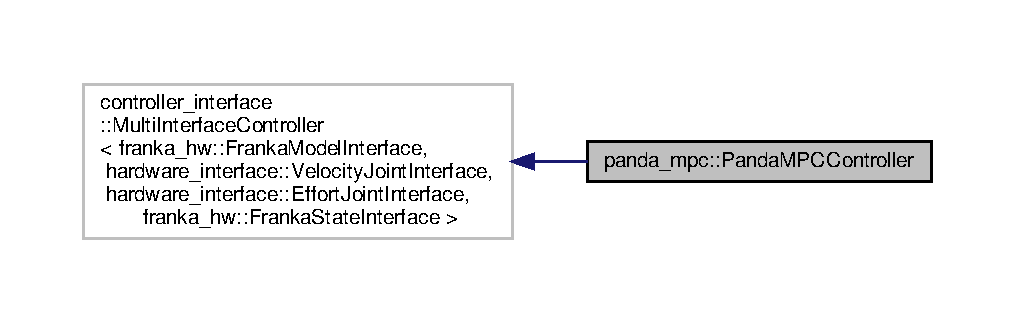
\includegraphics[width=350pt]{classpanda__mpc_1_1_panda_m_p_c_controller__inherit__graph}
\end{center}
\end{figure}


Collaboration diagram for panda\+\_\+mpc\+:\+:Panda\+M\+P\+C\+Controller\+:
\nopagebreak
\begin{figure}[H]
\begin{center}
\leavevmode
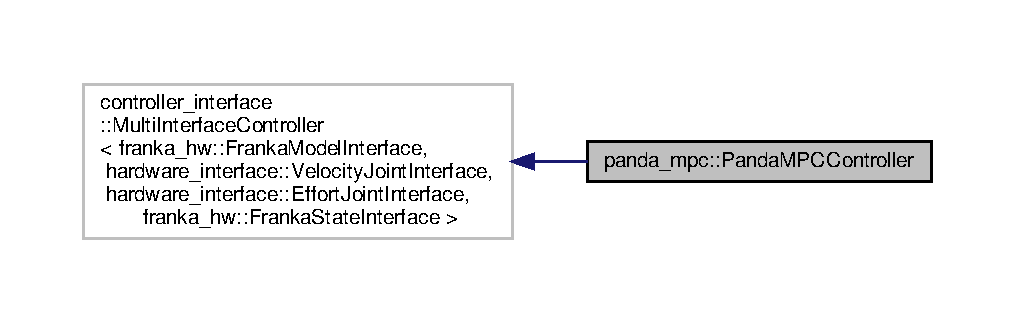
\includegraphics[width=350pt]{classpanda__mpc_1_1_panda_m_p_c_controller__coll__graph}
\end{center}
\end{figure}
\subsection*{Public Member Functions}
\begin{DoxyCompactItemize}
\item 
\mbox{\Hypertarget{classpanda__mpc_1_1_panda_m_p_c_controller_ae8d43af1f86cb114fd2d46b96104e5a0}\label{classpanda__mpc_1_1_panda_m_p_c_controller_ae8d43af1f86cb114fd2d46b96104e5a0}} 
bool \hyperlink{classpanda__mpc_1_1_panda_m_p_c_controller_ae8d43af1f86cb114fd2d46b96104e5a0}{init} (hardware\+\_\+interface\+::\+Robot\+HW $\ast$robot\+\_\+hw, ros\+::\+Node\+Handle \&node\+\_\+handle) override
\begin{DoxyCompactList}\small\item\em Franka Panda initialization routine. \end{DoxyCompactList}\item 
\mbox{\Hypertarget{classpanda__mpc_1_1_panda_m_p_c_controller_a70fc2fe27bc42c3b66740b0399feeb5e}\label{classpanda__mpc_1_1_panda_m_p_c_controller_a70fc2fe27bc42c3b66740b0399feeb5e}} 
void \hyperlink{classpanda__mpc_1_1_panda_m_p_c_controller_a70fc2fe27bc42c3b66740b0399feeb5e}{starting} (const ros\+::\+Time \&) override
\begin{DoxyCompactList}\small\item\em Franka Panda starting routine. \end{DoxyCompactList}\item 
\mbox{\Hypertarget{classpanda__mpc_1_1_panda_m_p_c_controller_a17e37eded424f2e5460dae0d5a5eea02}\label{classpanda__mpc_1_1_panda_m_p_c_controller_a17e37eded424f2e5460dae0d5a5eea02}} 
void \hyperlink{classpanda__mpc_1_1_panda_m_p_c_controller_a17e37eded424f2e5460dae0d5a5eea02}{update} (const ros\+::\+Time \&, const ros\+::\+Duration \&period) override
\begin{DoxyCompactList}\small\item\em Franka Panda controller update routine. \end{DoxyCompactList}\end{DoxyCompactItemize}


The documentation for this class was generated from the following files\+:\begin{DoxyCompactItemize}
\item 
/home/zheng/catkin\+\_\+ws/src/panda\+\_\+mpc/include/robot/panda\+\_\+controller.\+h\item 
/home/zheng/catkin\+\_\+ws/src/panda\+\_\+mpc/src/panda\+\_\+controller.\+cpp\end{DoxyCompactItemize}

\hypertarget{classgazebo_1_1_panda_simulation}{}\section{gazebo\+:\+:Panda\+Simulation Class Reference}
\label{classgazebo_1_1_panda_simulation}\index{gazebo\+::\+Panda\+Simulation@{gazebo\+::\+Panda\+Simulation}}


Inheritance diagram for gazebo\+:\+:Panda\+Simulation\+:\nopagebreak
\begin{figure}[H]
\begin{center}
\leavevmode
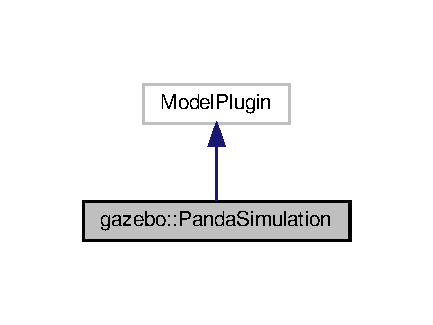
\includegraphics[width=208pt]{classgazebo_1_1_panda_simulation__inherit__graph}
\end{center}
\end{figure}


Collaboration diagram for gazebo\+:\+:Panda\+Simulation\+:
\nopagebreak
\begin{figure}[H]
\begin{center}
\leavevmode
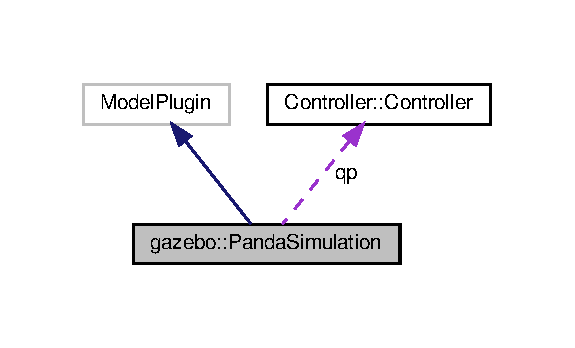
\includegraphics[width=276pt]{classgazebo_1_1_panda_simulation__coll__graph}
\end{center}
\end{figure}
\subsection*{Public Member Functions}
\begin{DoxyCompactItemize}
\item 
\mbox{\Hypertarget{classgazebo_1_1_panda_simulation_ac1c50ed325e6f05209f0586593bed996}\label{classgazebo_1_1_panda_simulation_ac1c50ed325e6f05209f0586593bed996}} 
void {\bfseries Load} (physics\+::\+Model\+Ptr model, sdf\+::\+Element\+Ptr)
\item 
\mbox{\Hypertarget{classgazebo_1_1_panda_simulation_acfea2cf28afae4d972657ba5a2ac3fce}\label{classgazebo_1_1_panda_simulation_acfea2cf28afae4d972657ba5a2ac3fce}} 
bool {\bfseries load\+World} ()
\item 
\mbox{\Hypertarget{classgazebo_1_1_panda_simulation_ae55621ade589fa28441d6a6e1156161d}\label{classgazebo_1_1_panda_simulation_ae55621ade589fa28441d6a6e1156161d}} 
double {\bfseries get\+Iterations} ()
\item 
\mbox{\Hypertarget{classgazebo_1_1_panda_simulation_ac4aff98571705909a74bb7f65a40a8ec}\label{classgazebo_1_1_panda_simulation_ac4aff98571705909a74bb7f65a40a8ec}} 
void {\bfseries print} () const
\item 
\mbox{\Hypertarget{classgazebo_1_1_panda_simulation_a6207a68e3517f272140b2054da202227}\label{classgazebo_1_1_panda_simulation_a6207a68e3517f272140b2054da202227}} 
void {\bfseries print\+State} () const
\item 
\mbox{\Hypertarget{classgazebo_1_1_panda_simulation_a0012e76a974d6f4abd83ea1cd9afaa4b}\label{classgazebo_1_1_panda_simulation_a0012e76a974d6f4abd83ea1cd9afaa4b}} 
const Eigen\+::\+Vector3d \& {\bfseries get\+Gravity} () const
\item 
\mbox{\Hypertarget{classgazebo_1_1_panda_simulation_ae433d080b82acb85649dd7b4b303698e}\label{classgazebo_1_1_panda_simulation_ae433d080b82acb85649dd7b4b303698e}} 
const std\+::vector$<$ std\+::string $>$ \& {\bfseries get\+Actuated\+Joint\+Names} () const
\item 
\mbox{\Hypertarget{classgazebo_1_1_panda_simulation_a053ccf46d079a7f0e345d2588994fc2b}\label{classgazebo_1_1_panda_simulation_a053ccf46d079a7f0e345d2588994fc2b}} 
const Eigen\+::\+Matrix$<$ double, 6, 1 $>$ \& {\bfseries get\+Base\+Velocity} () const
\item 
\mbox{\Hypertarget{classgazebo_1_1_panda_simulation_a8631b9b7d6294b6d78b0ce346c6f9ebb}\label{classgazebo_1_1_panda_simulation_a8631b9b7d6294b6d78b0ce346c6f9ebb}} 
const Eigen\+::\+Affine3d \& {\bfseries get\+World\+To\+Base\+Transform} () const
\item 
\mbox{\Hypertarget{classgazebo_1_1_panda_simulation_a77e7229b268b3c017a3978b665590cf5}\label{classgazebo_1_1_panda_simulation_a77e7229b268b3c017a3978b665590cf5}} 
const Eigen\+::\+Vector\+Xd \& {\bfseries get\+Joint\+Positions} () const
\item 
\mbox{\Hypertarget{classgazebo_1_1_panda_simulation_aa2c2a0942fb5c92963f5346ca43c41db}\label{classgazebo_1_1_panda_simulation_aa2c2a0942fb5c92963f5346ca43c41db}} 
const Eigen\+::\+Vector\+Xd \& {\bfseries get\+Joint\+Velocities} () const
\item 
\mbox{\Hypertarget{classgazebo_1_1_panda_simulation_a0894b02fce85f67fc738d6b39f003ffb}\label{classgazebo_1_1_panda_simulation_a0894b02fce85f67fc738d6b39f003ffb}} 
void {\bfseries set\+Joint\+Gravity\+Torques} (const Eigen\+::\+Vector\+Xd \&gravity\+\_\+torques)
\item 
\mbox{\Hypertarget{classgazebo_1_1_panda_simulation_afd74aa25a079896d404a7988179535d8}\label{classgazebo_1_1_panda_simulation_afd74aa25a079896d404a7988179535d8}} 
const Eigen\+::\+Vector\+Xd \& {\bfseries get\+Joint\+External\+Torques} () const
\item 
\mbox{\Hypertarget{classgazebo_1_1_panda_simulation_ad122946ad9e69b5932855f15df6a3b9c}\label{classgazebo_1_1_panda_simulation_ad122946ad9e69b5932855f15df6a3b9c}} 
const Eigen\+::\+Vector\+Xd \& {\bfseries get\+Joint\+Measured\+Torques} () const
\item 
\mbox{\Hypertarget{classgazebo_1_1_panda_simulation_a562e9bbacd575381fe7582dcd6dd4d8b}\label{classgazebo_1_1_panda_simulation_a562e9bbacd575381fe7582dcd6dd4d8b}} 
void {\bfseries set\+Joint\+Torque\+Command} (const Eigen\+::\+Vector\+Xd \&joint\+\_\+torque\+\_\+command)
\item 
\mbox{\Hypertarget{classgazebo_1_1_panda_simulation_a6b1958c7de3707dc3984e0ba70f34d2e}\label{classgazebo_1_1_panda_simulation_a6b1958c7de3707dc3984e0ba70f34d2e}} 
const std\+::string \& {\bfseries get\+Name} () const
\item 
\mbox{\Hypertarget{classgazebo_1_1_panda_simulation_ab1fde66312c68f0f626c65846b9a5897}\label{classgazebo_1_1_panda_simulation_ab1fde66312c68f0f626c65846b9a5897}} 
const std\+::string \& {\bfseries get\+Base\+Name} ()
\item 
\mbox{\Hypertarget{classgazebo_1_1_panda_simulation_ae7379a3f13baabc530055ba8140d82b3}\label{classgazebo_1_1_panda_simulation_ae7379a3f13baabc530055ba8140d82b3}} 
void {\bfseries set\+Brakes} (bool enable)
\item 
\mbox{\Hypertarget{classgazebo_1_1_panda_simulation_a0fac8fcf06af7b21bb7a68f98c494e3c}\label{classgazebo_1_1_panda_simulation_a0fac8fcf06af7b21bb7a68f98c494e3c}} 
int {\bfseries get\+N\+Dof} () const
\item 
\mbox{\Hypertarget{classgazebo_1_1_panda_simulation_aaabec68606f677cfa46df91a17f1d948}\label{classgazebo_1_1_panda_simulation_aaabec68606f677cfa46df91a17f1d948}} 
void {\bfseries world\+Update\+Begin} ()
\item 
\mbox{\Hypertarget{classgazebo_1_1_panda_simulation_a16ec7f132866d2abcd0780d56178953e}\label{classgazebo_1_1_panda_simulation_a16ec7f132866d2abcd0780d56178953e}} 
void {\bfseries execute\+After\+World\+Update} (std\+::function$<$ void(uint32\+\_\+t, double, double)$>$ callback)
\item 
\mbox{\Hypertarget{classgazebo_1_1_panda_simulation_a45a8b9835469071f56b7943b80b05909}\label{classgazebo_1_1_panda_simulation_a45a8b9835469071f56b7943b80b05909}} 
void {\bfseries world\+Update\+End} ()
\item 
\mbox{\Hypertarget{classgazebo_1_1_panda_simulation_a2db6dca2d21fa4a60f150ae05b3732e6}\label{classgazebo_1_1_panda_simulation_a2db6dca2d21fa4a60f150ae05b3732e6}} 
void {\bfseries set\+Model\+Configuration} (const std\+::vector$<$ std\+::string $>$ \&joint\+\_\+names, const std\+::vector$<$ double $>$ \&joint\+\_\+positions)
\end{DoxyCompactItemize}
\subsection*{Public Attributes}
\begin{DoxyCompactItemize}
\item 
\mbox{\Hypertarget{classgazebo_1_1_panda_simulation_a6edfbdee5dbbc7fc7c27e3355306a25c}\label{classgazebo_1_1_panda_simulation_a6edfbdee5dbbc7fc7c27e3355306a25c}} 
Eigen\+::\+Vector\+Xd {\bfseries q}
\item 
\mbox{\Hypertarget{classgazebo_1_1_panda_simulation_a05b96d5dba5c3dace05fb7adc113c65e}\label{classgazebo_1_1_panda_simulation_a05b96d5dba5c3dace05fb7adc113c65e}} 
Eigen\+::\+Vector\+Xd {\bfseries qd}
\item 
\mbox{\Hypertarget{classgazebo_1_1_panda_simulation_ad4a114a61d723ccc689953771bc4a759}\label{classgazebo_1_1_panda_simulation_ad4a114a61d723ccc689953771bc4a759}} 
Eigen\+::\+Vector\+Xd {\bfseries joint\+\_\+command\+\_\+}
\item 
\mbox{\Hypertarget{classgazebo_1_1_panda_simulation_aca3cc95ca503ca10c2a4a7db8d89badd}\label{classgazebo_1_1_panda_simulation_aca3cc95ca503ca10c2a4a7db8d89badd}} 
std\+::vector$<$ std\+::string $>$ {\bfseries jn}
\item 
\mbox{\Hypertarget{classgazebo_1_1_panda_simulation_a3de095d48a03744458f3fbfd0586a845}\label{classgazebo_1_1_panda_simulation_a3de095d48a03744458f3fbfd0586a845}} 
std\+::vector$<$ double $>$ {\bfseries jp}
\item 
\mbox{\Hypertarget{classgazebo_1_1_panda_simulation_a66dff3094f71bed56945d21fbaa18c6e}\label{classgazebo_1_1_panda_simulation_a66dff3094f71bed56945d21fbaa18c6e}} 
gazebo\+::common\+::\+Time {\bfseries time}
\item 
\mbox{\Hypertarget{classgazebo_1_1_panda_simulation_a7dfa6f32365b8bf6c0ca1eec146bc012}\label{classgazebo_1_1_panda_simulation_a7dfa6f32365b8bf6c0ca1eec146bc012}} 
gazebo\+::common\+::\+P\+ID {\bfseries pid}
\item 
\mbox{\Hypertarget{classgazebo_1_1_panda_simulation_af8387bd9dce6a8c0ad049caba4f33999}\label{classgazebo_1_1_panda_simulation_af8387bd9dce6a8c0ad049caba4f33999}} 
int {\bfseries i}
\item 
\mbox{\Hypertarget{classgazebo_1_1_panda_simulation_a1a27740a962e526889dd0a071e5eb55f}\label{classgazebo_1_1_panda_simulation_a1a27740a962e526889dd0a071e5eb55f}} 
ros\+::\+Duration {\bfseries period}
\item 
\mbox{\Hypertarget{classgazebo_1_1_panda_simulation_aa4fc0613df28f9c75d9d5170a0c67f9b}\label{classgazebo_1_1_panda_simulation_aa4fc0613df28f9c75d9d5170a0c67f9b}} 
ros\+::\+Duration {\bfseries elapsed\+\_\+time\+\_\+}
\item 
\mbox{\Hypertarget{classgazebo_1_1_panda_simulation_a1ceb842453aa9714366432134bbd0941}\label{classgazebo_1_1_panda_simulation_a1ceb842453aa9714366432134bbd0941}} 
physics\+::\+Joint\+\_\+V {\bfseries joints\+\_\+}
\item 
\mbox{\Hypertarget{classgazebo_1_1_panda_simulation_a40684c917baf05e392e38a3bc6046552}\label{classgazebo_1_1_panda_simulation_a40684c917baf05e392e38a3bc6046552}} 
physics\+::\+Link\+\_\+V {\bfseries links\+\_\+}
\item 
\mbox{\Hypertarget{classgazebo_1_1_panda_simulation_a471c574062e04e6fe9fa38f1df934308}\label{classgazebo_1_1_panda_simulation_a471c574062e04e6fe9fa38f1df934308}} 
std\+::string {\bfseries name\+\_\+}
\item 
\mbox{\Hypertarget{classgazebo_1_1_panda_simulation_a2b22a3074d11024290c1a7906f9ca954}\label{classgazebo_1_1_panda_simulation_a2b22a3074d11024290c1a7906f9ca954}} 
int {\bfseries ndof\+\_\+} = 0
\item 
\mbox{\Hypertarget{classgazebo_1_1_panda_simulation_a58b09cb4e1249e6f677a625f890c429a}\label{classgazebo_1_1_panda_simulation_a58b09cb4e1249e6f677a625f890c429a}} 
Eigen\+::\+Vector\+Xd {\bfseries current\+\_\+joint\+\_\+positions\+\_\+}
\item 
\mbox{\Hypertarget{classgazebo_1_1_panda_simulation_a0ec51844867731f643b09193ab631ab8}\label{classgazebo_1_1_panda_simulation_a0ec51844867731f643b09193ab631ab8}} 
Eigen\+::\+Vector\+Xd {\bfseries current\+\_\+joint\+\_\+velocities\+\_\+}
\item 
\mbox{\Hypertarget{classgazebo_1_1_panda_simulation_a9e864ba4666585ecece910b8e217f9f8}\label{classgazebo_1_1_panda_simulation_a9e864ba4666585ecece910b8e217f9f8}} 
Eigen\+::\+Vector\+Xd {\bfseries joint\+\_\+gravity\+\_\+torques\+\_\+}
\item 
\mbox{\Hypertarget{classgazebo_1_1_panda_simulation_a74167069fd53ea672b39d7d9b96d18e1}\label{classgazebo_1_1_panda_simulation_a74167069fd53ea672b39d7d9b96d18e1}} 
Eigen\+::\+Vector\+Xd {\bfseries current\+\_\+joint\+\_\+external\+\_\+torques\+\_\+}
\item 
\mbox{\Hypertarget{classgazebo_1_1_panda_simulation_a76bbdab784df342f7042aa9bd49c2310}\label{classgazebo_1_1_panda_simulation_a76bbdab784df342f7042aa9bd49c2310}} 
Eigen\+::\+Vector\+Xd {\bfseries joint\+\_\+torque\+\_\+command\+\_\+}
\item 
\mbox{\Hypertarget{classgazebo_1_1_panda_simulation_a8f26d9d2d1060a9ebf6841bf0f5eac5f}\label{classgazebo_1_1_panda_simulation_a8f26d9d2d1060a9ebf6841bf0f5eac5f}} 
Eigen\+::\+Vector\+Xd {\bfseries current\+\_\+joint\+\_\+measured\+\_\+torques\+\_\+}
\item 
\mbox{\Hypertarget{classgazebo_1_1_panda_simulation_ae2ff65eb458903adeb3a94e6b3135211}\label{classgazebo_1_1_panda_simulation_ae2ff65eb458903adeb3a94e6b3135211}} 
gazebo\+::event\+::\+Connection\+Ptr {\bfseries world\+\_\+begin\+\_\+}
\item 
\mbox{\Hypertarget{classgazebo_1_1_panda_simulation_a0392f81c0a1af939a801b0144a37339b}\label{classgazebo_1_1_panda_simulation_a0392f81c0a1af939a801b0144a37339b}} 
gazebo\+::event\+::\+Connection\+Ptr {\bfseries world\+\_\+end\+\_\+}
\item 
\mbox{\Hypertarget{classgazebo_1_1_panda_simulation_a5cf10e5600f5ee5cfec74f78d757a453}\label{classgazebo_1_1_panda_simulation_a5cf10e5600f5ee5cfec74f78d757a453}} 
std\+::vector$<$ std\+::string $>$ {\bfseries actuated\+\_\+joint\+\_\+names\+\_\+}
\item 
\mbox{\Hypertarget{classgazebo_1_1_panda_simulation_ad25690d987147052b2d0c1ea20a06646}\label{classgazebo_1_1_panda_simulation_ad25690d987147052b2d0c1ea20a06646}} 
physics\+::\+Model\+Ptr {\bfseries model\+\_\+}
\item 
\mbox{\Hypertarget{classgazebo_1_1_panda_simulation_ace15eb1ae41c098028571966144053a5}\label{classgazebo_1_1_panda_simulation_ace15eb1ae41c098028571966144053a5}} 
Eigen\+::\+Vector3d {\bfseries gravity\+\_\+vector\+\_\+}
\item 
\mbox{\Hypertarget{classgazebo_1_1_panda_simulation_aa167df29f8a9c183c84e3d29cfc52b13}\label{classgazebo_1_1_panda_simulation_aa167df29f8a9c183c84e3d29cfc52b13}} 
Eigen\+::\+Matrix$<$ double, 6, 1 $>$ {\bfseries current\+\_\+base\+\_\+vel\+\_\+}
\item 
\mbox{\Hypertarget{classgazebo_1_1_panda_simulation_a70f1bd58bf3285e80d7c9e1344e26980}\label{classgazebo_1_1_panda_simulation_a70f1bd58bf3285e80d7c9e1344e26980}} 
Eigen\+::\+Affine3d {\bfseries current\+\_\+world\+\_\+to\+\_\+base\+\_\+}
\item 
\mbox{\Hypertarget{classgazebo_1_1_panda_simulation_acd5c9922b7dc10e96900954d3e5888b2}\label{classgazebo_1_1_panda_simulation_acd5c9922b7dc10e96900954d3e5888b2}} 
std\+::string {\bfseries base\+\_\+name\+\_\+}
\item 
\mbox{\Hypertarget{classgazebo_1_1_panda_simulation_a3c2c1305ac89b2033976946505894254}\label{classgazebo_1_1_panda_simulation_a3c2c1305ac89b2033976946505894254}} 
std\+::function$<$ void(uint32\+\_\+t, double, double)$>$ {\bfseries callback\+\_\+}
\item 
\mbox{\Hypertarget{classgazebo_1_1_panda_simulation_ac78dfbd642bdd959ae98ea0b4b7009e6}\label{classgazebo_1_1_panda_simulation_ac78dfbd642bdd959ae98ea0b4b7009e6}} 
bool {\bfseries brakes\+\_\+}
\item 
\mbox{\Hypertarget{classgazebo_1_1_panda_simulation_a7969b2892ab06a98984c069b3724fa3e}\label{classgazebo_1_1_panda_simulation_a7969b2892ab06a98984c069b3724fa3e}} 
double {\bfseries old\+\_\+time}
\item 
\mbox{\Hypertarget{classgazebo_1_1_panda_simulation_aa09a367c75567516386b5aabe77aa8e8}\label{classgazebo_1_1_panda_simulation_aa09a367c75567516386b5aabe77aa8e8}} 
\hyperlink{class_controller_1_1_controller}{Controller\+::\+Controller} {\bfseries qp}
\item 
\mbox{\Hypertarget{classgazebo_1_1_panda_simulation_ab0c67a1a87c61b8edc035cdc1c57d922}\label{classgazebo_1_1_panda_simulation_ab0c67a1a87c61b8edc035cdc1c57d922}} 
std\+::string {\bfseries control\+\_\+level}
\item 
\mbox{\Hypertarget{classgazebo_1_1_panda_simulation_a1628fdf512b4f9984e138268f27be602}\label{classgazebo_1_1_panda_simulation_a1628fdf512b4f9984e138268f27be602}} 
ros\+::\+Publisher {\bfseries joint\+\_\+states\+\_\+pub\+\_\+}
\item 
\mbox{\Hypertarget{classgazebo_1_1_panda_simulation_a9c8b4023a0f65f89aeab2ab97ee761fb}\label{classgazebo_1_1_panda_simulation_a9c8b4023a0f65f89aeab2ab97ee761fb}} 
sensor\+\_\+msgs\+::\+Joint\+State {\bfseries joint\+\_\+states\+\_\+}
\end{DoxyCompactItemize}


The documentation for this class was generated from the following file\+:\begin{DoxyCompactItemize}
\item 
/home/zheng/catkin\+\_\+ws/src/panda\+\_\+mpc/src/panda\+\_\+simulation.\+cpp\end{DoxyCompactItemize}

%--- End generated contents ---

% Index
\backmatter
\newpage
\phantomsection
\clearemptydoublepage
\addcontentsline{toc}{chapter}{Index}
\printindex

\end{document}
